

\chapter{Using Deep Learning to Detect Technical Debt}

We aim to create a system that automatically detects technical debt in a class method. To achieve this goal, we took the following three steps: dataset creation, classification and hyperparameter tuning.
The dataset was automatically created by mining and processing open-source projects histories. It is a balanced dataset by construction and the two classes are referred to as: SATD and fixed.

We initially identify technical debt through the presence of SATD in the comments of the source code, using keyword labels pattern matching \cite{potdar2014exploratory} \cite{rantala2020prevalence}.
The identification of a SATD/fixed method pair is based on a strong assumption: when the SATD comment disappears, due to a commit, we suppose that the technical debt is fixed; so, we regard the new code as TD-free, belonging to the fixed class.
% detail: describe the circumstances where we reject this hypotheses
The classifier is a neural network capable of representing snippets of code with a fixed-length vector, conceptually similar to how word2vec works. The learned vector representation (code embedding) is associated with a semantic label (i.e. SATD or fixed).
Lastly, to increase the performance of the system we select a set of hyperparameters and perform a distributed grid search for tuning their values. The rest of this chapter explains each part in greater detail.

%3.1
\section{Mining SATD Instances and their Fixes}

These are the fundamental activities involved in the creation of the dataset:
\begin{itemize}
    \item Github repository URL mining: using Github API, we extracted 248,872 projects' URL matching our search profile.
    \item Repository cloning and filtering: some projects can be discarded only after the commit history is available for a precursory analysis to determine if a project qualifies for the next activity.
    \item Commit history processing: the directed acyclic graph of the commits is traversed and the source code is parsed in search of acceptable SATD/fixed pair.
\end{itemize}

The following sections describe these activities in detail.

\subsection{Github repository url mining}
We know from experience and the literature that the concentration of SATD is very low \cite{bavota2016large} \cite{maldonado2015detecting} \cite{potdar2014exploratory}, for this reason we created a dataset from an initial set of open-source projects as big as possible. 
The search was conducted for all public Java GitHub repositories in a 20 years time window (from 2000 to 2019). 
The retrieval process of this URLs list was challenging in itself. We dealt and solved the following issues:
\begin{enumerate}
    \item GitHub search API limit of 1000 hits.
    \item GitHub search API number of request per minute maximum quota.
    \item Filtering to remove low-quality repositories
    \item Unexpected interruptions
\end{enumerate}
We addressed the first issue with two different intertwined phases of queries: probe and harvest. The probe requested only the number of the repositories that were created in a specific time window; if the number exceeds the 1000 limit, it iteratively divides the probe query into two sub-queries using half of the time window for each and adds them to the job queue.
It was not enough to specify the day interval in the query; the time of the day was also needed because in the recent years there are multiple instances of more than 1000 repositories created in a single day.

The second issue was solved using an authentication token, as specified by the GitHub documentation.

The third issue was the reason we switched to the GitHub GraphQL API; we quickly realized that the total number of repositories in the selected period was more than seven million and we needed a way to trim down the list to those most meaningful repositories. We empirically defined, through a trial and error process, a metric to keep those repositories with a good likelihood to contain \textit{higher quality source code}. 
The GraphQL Repository API can be queried to return additional information; for each repository, we requested the issue count and the commit count so to discard quickly those with less or equal than 100 commits and 100 issues. It must be noted that the GraphQL query automatically excluded some repositories because of atypical structures (e.g. Subversion to git converts and repositories with non-standard naming). 

The last issue affects all long-running processes: unexpected interruptions, e.g. network outages, program crashes, API service unavailability. To fix these problems, all failed queries are repeated for a maximum of 50 times, then the program is halted with an exception. 
The program can recover from a crash because every query is cached to a file; when a query is issued and the cache is present the network request is skipped and the file content is used instead. This was important because the URLs mining execution took roughly 150 hours and a system to reuse past expended resources were needed.

The URLs mining tool creates two text files: one with the complete list and one with the URLs that match our acceptance criteria. Both files contain the following columns:

\begin{itemize}
    \item Repository creation date.
    \item User name and repository name.
    \item Issue count.
    \item Commit count.
\end{itemize}

The total number of URLs retrieved was roughly seven million but we accepted only a subset of them: around 250 thousand repositories.

% expand on cache because it takes a few days to mine all URLs





\subsection{Repository cloning and filtering}
% 250.000 cloni
% esclusione repository Android OS , 300.000 commits 
% spazio su disco e cancellazione on the go
% the processing was done just after one repo was cloned 
% description next section
This section describes the process of cloning 250 thousand repositories and applying further filtering. 

The repository clone task was conducted without the checkout, i.e. only the commit history was downloaded without creating the working copy for the last commit. This approach saved disk space and processing time, particularly when the last commit contained a high number of files. 

Once the repository was locally accessible, using the library JGit\footnote{https://www.eclipse.org/jgit/}, we tested the presence of a few files that indicated an Android OS project; if it was the case, the repository was rejected.
The problems related to the Android OS was that there were more than 1,700 forks/clones and those repositories counted between 300,000 and 550,000 commits; it is one of the biggest project encountered in this endeavour and it posed a significant bottleneck to the commit history processing: traversing the commit tree could take a couple of days only for one Android OS repository.
The exclusion of Android OS in this phase was established only for performance reasons.

The general issue of detecting forked (i.e. duplicated) repositories will be better explained in the next section.



\subsection{Commit history processing}

This section describes the task of traversing all the commits of a repository and collecting the code snippets to our SATD/fixed dataset.

What we are generally looking for is a method body that is affected with SATD and after a commit is not affected by it anymore, i.e. the SATD was removed. What follows from it is that we do not need to blindly parse all the Java files but only those that are changed by a commit.

For each repository we iterate on every commit and every file change; but we care only of \textit{modify} type operations; we ignore the rest of git file change operations: add, delete, rename and copy.

At this stage we just have a pair of Java source code texts: the old version before the commit and the new after it; they are also called \textit{before image} and \textit{after image}. Next, we parse the before image and run the SATD detector; if hits are found, then we parse also the after image.

Now we tackle the previous explanation with a different abstraction level in mind: not from the source file point of view but at the method level. 
What we have is a list of methods affected by SATD coming from the before image and another list of methods created from the after image; we couple the items of these two lists by method name and accept as viable candidates only those pairs whose after image method is not affected with SATD. The following code implements the semantic described before (old stands for before image and new stands for after image):

\begin{center}
  \makebox[\textwidth]{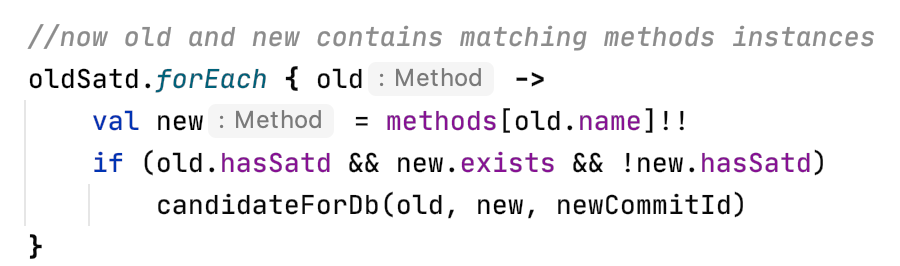
\includegraphics[width=0.7\columnwidth]{images/pairing_methods.png}}
\end{center}

There are a few considerations to ponder: 

\begin{itemize}
    \item The appearance order of the methods in the source code does not affect the process.
    \item When a method is removed it is automatically excluded through the lack of pairing between the two lists.
    \item The renamed methods are lost; they are treated as removed.
\end{itemize}

\noindent The rest of this section develops some aspects that were not fully explained before but that are important to the creation of the dataset.
\\
\\
\textbf{Keyword label pattern matching.} 
To detect the SATD, we use keyword label techniques using the 62 patterns reported by Potdar and Shihab \cite{potdar2014exploratory} (they are actually 63\footnote{http://users.encs.concordia.ca/~eshihab/data/ICSME2014/satd.html}). Out of these patterns we create regular expressions that are applied on all the source comments extracted with JavaParser.

We did an initial experiment to verify the effectiveness of those patterns and we excluded the following two: ``there is a problem'' and ``bail out''. After manually verifying roughly one hundred matches we noticed that those two patterns were often used as documentation in `catch' Java blocks and were not documenting SATD. The final list used in our tool is found in listing \ref{lst:patterns61}.


\textbf{Snippets preprocessing and cleaning.} \label{sec:cleaning} Every sample in the dataset contains the verbatim method source code pair (before image and after image). It also contains a new pair (called `clean') cleaned by all comments and string literals. The string cleaning process replaces all the non-null and non-empty strings to a constant: ``--\#\#string\#\#--''. In other words, the string type values are constrained to this set: null, empty value and ``--\#\#string\#\#--''.

\textbf{Precomputed features}
The neural model used in this thesis needs a specific representation for each code snippet (see section \ref{sec:code2vec_ast_paths} for details). The computation of such representation is resource expensive and we decided to store it in the database alongside with the sample (columns old\_clean\_features and new\_clean\_features).


\textbf{Handling forks and duplicated code.}
In our research we found that many repositories were duplicates or clones (GitHub keeps track of forks but do not track duplicates). 
We need to be very careful not to introduce noise in the dataset. To ensure a better quality for our samples we implemented the following steps:
\begin{itemize}
    \item We concatenated the clean images (before and after images) and computed the hash of such a string. This hash is stored in a database field with a unique index on it; this ensures that we do not have duplicated pairs.
    \item Two additional hashes are calculated: one for the clean before image and a second for the clean after image. Then we discard all pairs that are found having a hash in common between any before and after clean image hash; this ensures that we cannot have the same snippet in both before and after image.
    \item We did the same process as described in the previous point but applied to the precomputed features.
\end{itemize}

\textbf{Rejected snippets.} 
% see JavaMethodTest.kt
We implemented unit tests\footnote{https://github.com/simonegiacomelli/code2vec-satd-classifier/blob/master/satd-classifier/src/jvmTest/kotlin/satd/step2/JavaMethodTest.kt} to be sure to reject specific Java constructs that would pose issues for the pipeline. For example, methods containing inner named methods (explicit interface implementations) were discarded because the parser in code2vec recognized them as two distinct methods, which is not correct. 


\section{The Deep Learning Model}
The model described in this section is called code2vec \cite{alon2019code2vec}.
The following three sequential processes can be considered a chain that progressively transforms the source code into the desired target (i.e. the two classes SATD/fixed):
\begin{itemize}
    \item Decompose
    \item Aggregate
    \item Predict
\end{itemize}

\noindent Each of these steps can be viewed as a process that takes an input, creates an intermediate representation and generates an output for the next process.
In the rest of this section we give some details about each one of them and introduce some technical terms. 
\\
\\
\noindent \textbf{Decompose.} The input of this process is the source code. The output generated is a bag of path-context. The following list gives more detail on the process and the intermediate representations:

\begin{itemize}
    \item Parsing and creation of the abstract syntax tree (AST) of the method source code. 
    \item Extraction of all AST-paths (up to a fixed limit).
    \item Encoding of the AST-paths into a bag of context-vector.
    \item Transform each context-vector into a path-context (so to obtain a bag of path-context).
\end{itemize}

\noindent \textbf{Aggregate.} This process aggregates the bag of path-context (the output from the previous process) using an attention vector. The final result is a code-vector that represents the snippet of code as a continuous distributed vector, i.e. a `code embedding'.
\\
\\
\noindent \textbf{Predict.} The code-vector is fed to a fully connected neural network that performs the classification using the desired classes (i.e. SATD/fixed).
\\
\\
\noindent In the following sections we expand and dig deeper into these concepts.

% Here I want to explain briefly what are the fundamental pieces and how they interact (without pretending that the reader really understands, but to give the general idea)

\subsection{Representing code using AST-paths} \label{sec:code2vec_ast_paths}
This section describes how to capture semantic information from code snippets and create a representation that can be used to predict properties of the snippet, for example a label (e.g. SATD/fixed).
To better illustrate how the decomposition is done, we use the simple code snippet in listing \ref{lst:snippet_ast_code} as an example .

%AST of code snippet
\begin{lstlisting}[caption={Example code to show decomposition}, label={lst:snippet_ast_code},language=Java]

                            String METHOD_NAME() {
                              if(somePreCondition())
                                while(!completed())
                                   doWork();
                              return "ok";
                            }
                            
\end{lstlisting}

Using JavaParser\footnote{https://javaparser.org/} the AST is extracted from the source code; see an example in figure  \ref{fig:AST_graphviz}.


\begin{figure}
 \centering
 \resizebox{\columnwidth}{!}{
 \includesvg[]{images/AST_graphviz}
 }
 \caption[AST for listing \ref{lst:snippet_ast_code}.]{Abstract syntax tree of the source code presented in listing \ref{lst:snippet_ast_code}.}
 \label{fig:AST_graphviz}
\end{figure}

	
We identify three sets of node types in the AST: values, terminal and non-terminal nodes. Values are the leaves (this set is identified with $X$), terminal nodes are the immediate parent of a leaf and the rest are the non-terminal ones.
\textit{AST-path definition}: it is a path connecting two terminal nodes and it must include one non-terminal node which is a common ancestor of the two terminal nodes. 
The representation of the program is the \textit{set of all its AST-paths}. 

To wrap up this section, we explain the last AST-path in figure \ref{fig:AST_paths} and, for convenience, this AST-path is also reported here:

%AST-paths only last
\begin{center}
  \makebox[\textwidth]{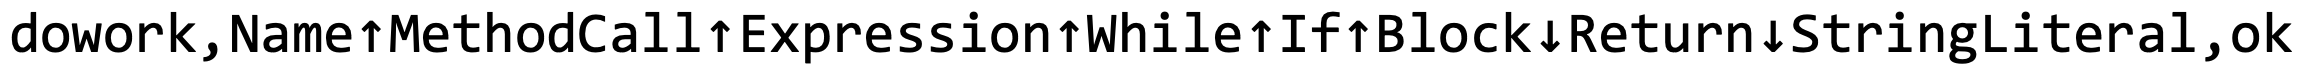
\includegraphics[width=\columnwidth]{images/AST_paths_last.png}}
\end{center}

The two value nodes are the first and the last words, `dowork' and `ok' respectively; the reader can also identify these leaf nodes in the bottom-right part of figure \ref{fig:AST_graphviz}.
The central part of the AST-path above is the connecting path between those two value nodes: it lists all the intermediate nodes and it also specifies the direction (up or down) one needs to take to traverse the tree. The common ancestor, for this example, is the intermediate node called `block'.

%AST-paths of code snippet
\begin{figure}
 \centering
 \resizebox{\columnwidth}{!}{
  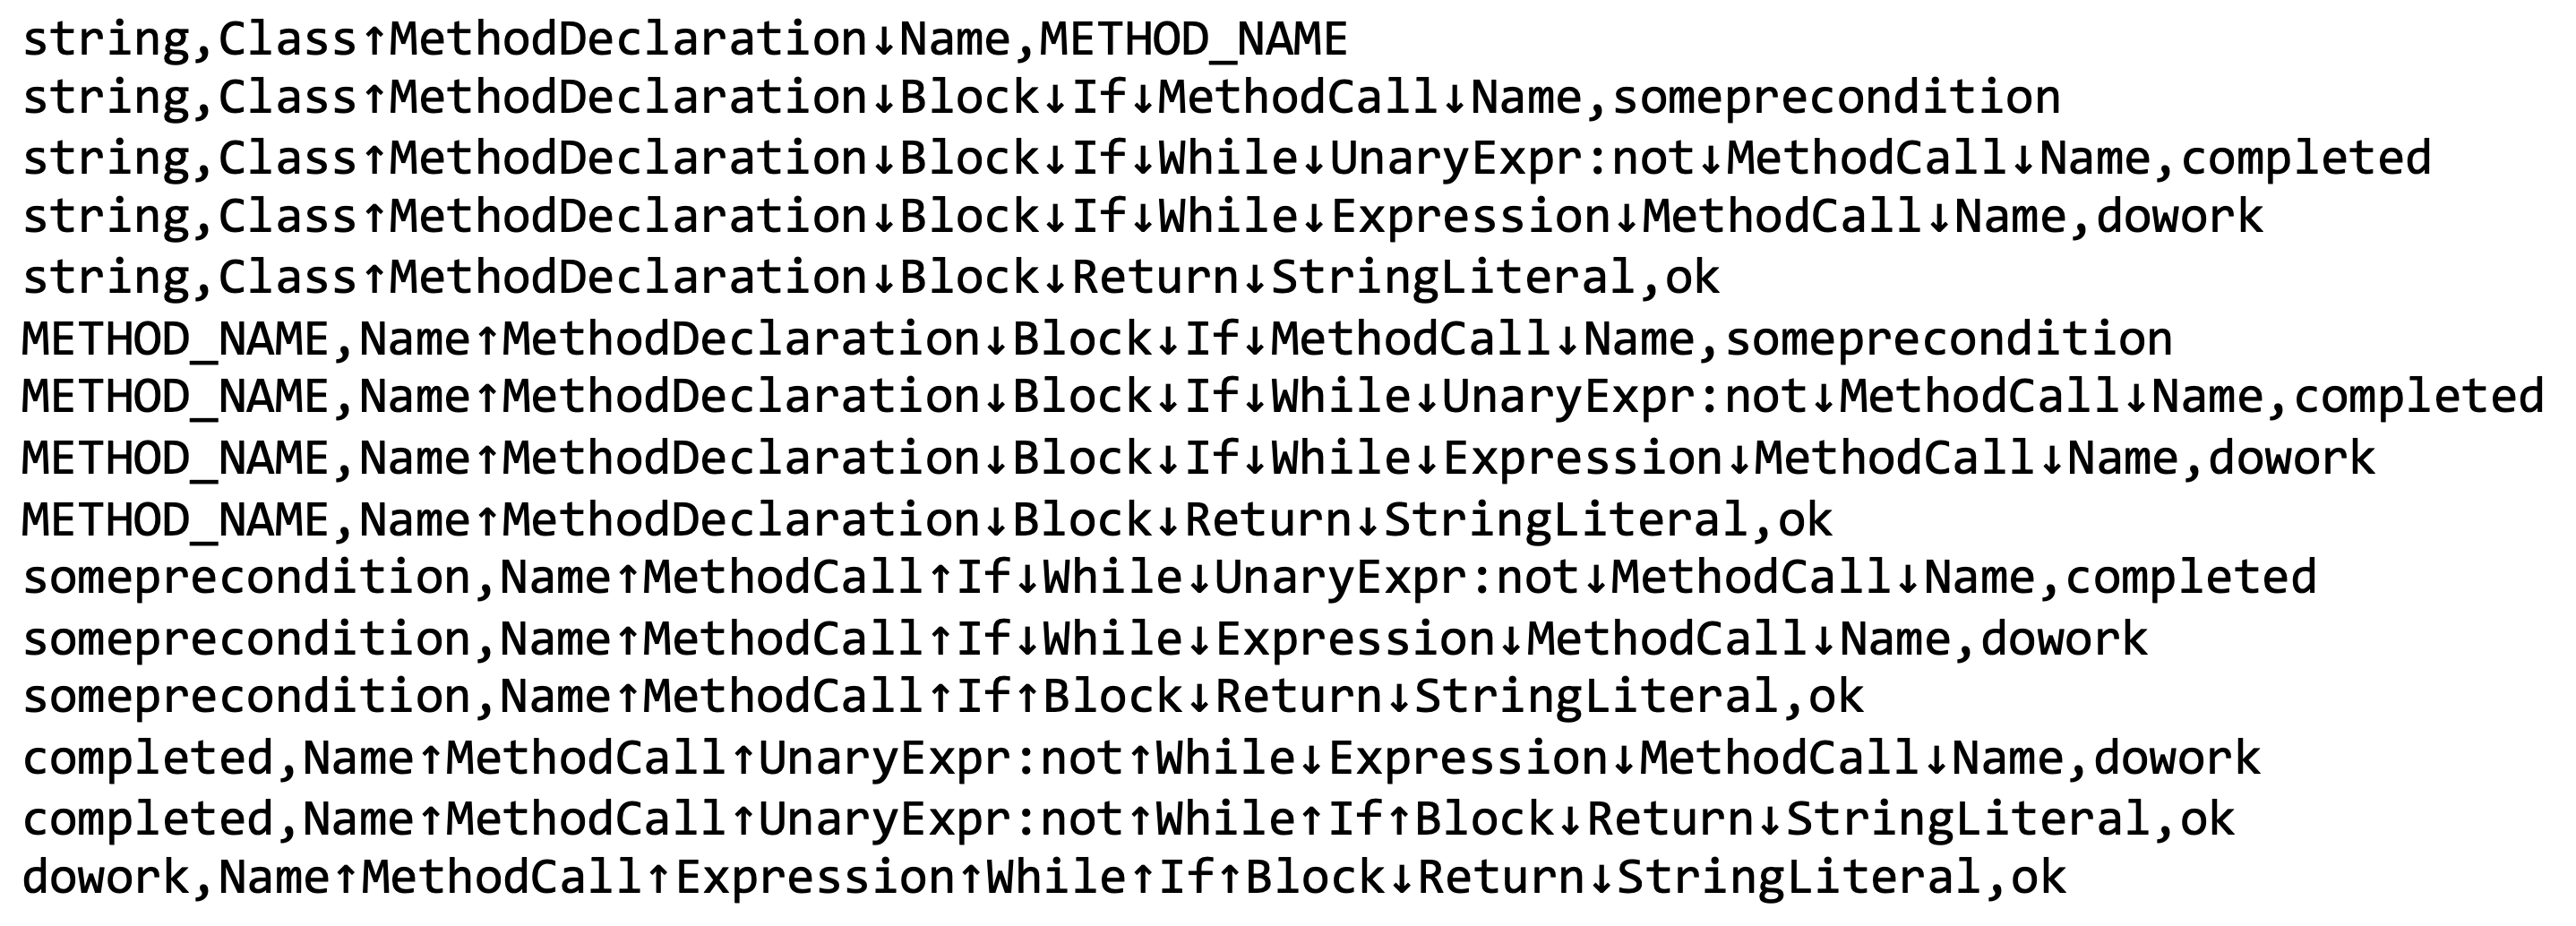
\includegraphics{images/AST_paths.png}
 }
 \caption[All AST-paths for listing \ref{lst:snippet_ast_code}.]{AST-paths of listing \ref{lst:snippet_ast_code}.}
    \label{fig:AST_paths}
\end{figure}

% here I go into details on the first decomposition/representation of the code snippets into fixed-length vectors

What is seen in figure \ref{fig:AST_paths} is a bag of context-paths (another name for the set of all AST-paths) and it is the representation for the code snippet. The following section explains how these AST-paths are transformed into fixed-length vectors.

\subsection{Context-vector}
%how many OOV? 
%https://github.com/tech-srl/code2vec/blob/c98e8f786b7262e56c93e520d039fb7aa5d0f7ef/vocabularies.py#L123

A context-vector $c_i$ is the vector representation for an AST-path. The process of transformation is applied to all AST-paths producing a bag of context-vectors.
The following picture shows how the context-vector is formed:

\begin{center}
  \makebox[\textwidth]{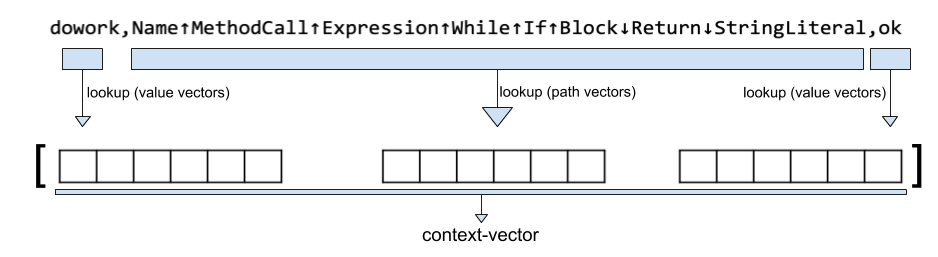
\includegraphics[width=\columnwidth]{images/context_vector.png}}
\end{center}

To explain the picture above we need to introduce two matrices:
\begin{align*} 
 value\_vocab \in \mathbb{R}^{|X| \times d}
\\
    path\_vocab \in \mathbb{R}^{|P| \times d}
\end{align*}
% \begin{itemize}
%     \item value\_vocab $\in \mathbb{R}^{|X| \times d}$
%     \item path\_vocab $\in \mathbb{R}^{|P| \times d}$
% \end{itemize}

The embedding size $d$ is a hyperparameter. $X$ is the set of values of the AST terminals that were observed during training; in our recurring example this set is composed of: string, METHOD\_NAME, someprecondition, completed, dowork and ok. 
$P$ is the set of all AST-paths across all snippets.

These matrices are initialized randomly and are learned by the model during the training.
An embedding (either from value\_vocab or path\_vocab) is looked up selecting the appropriate row in its matrix.

The previous notions tell us that:
\begin{align*} 
c_i \in  \mathbb{R}^{3 d}
\end{align*}

The two matrices value\_vocab and path\_vocab do not need to be of the same width $d$ but for convenience it was chosen so.

\subsection{Path-context}
The previous section describes the definition of the context-vector $c_i$. Applying a fully connected layer to it we obtain the path-context vector $\widetilde{c}_i$, also called combined context-vector. The following equation describes the computation of this layer:

\begin{align*} 
\widetilde{c}_i = \tanh( W \cdot c_i )
\end{align*}
where $W$ is the weight matrix and
\begin{align*} 
W \in  \mathbb{R}^{d \times 3 d}
\end{align*}

The height of $W$ is for convenience of the same size as before ($d$); it does not need to be strictly so: it can also be of different height.
One other way to look at this layer is that it compresses the context-vector $c_i$ of size $3d$ into a combined context-vector of size $d$.

\subsection{Attention mechanism and the code-vector} \label{sec:attention_code_vector}
The previous section left us with a set of path-contexts. The goal of this part of the model is to combine them all into a code-vector.
This step employs an attention vector $a$ (see figure \ref{fig:code2vec_arch}; it can be described as a weighted average that . The weights are initialized randomly and learned with respect to the bag of path-contexts. 


\begin{figure}
 \centering
 \resizebox{\columnwidth}{!}{
  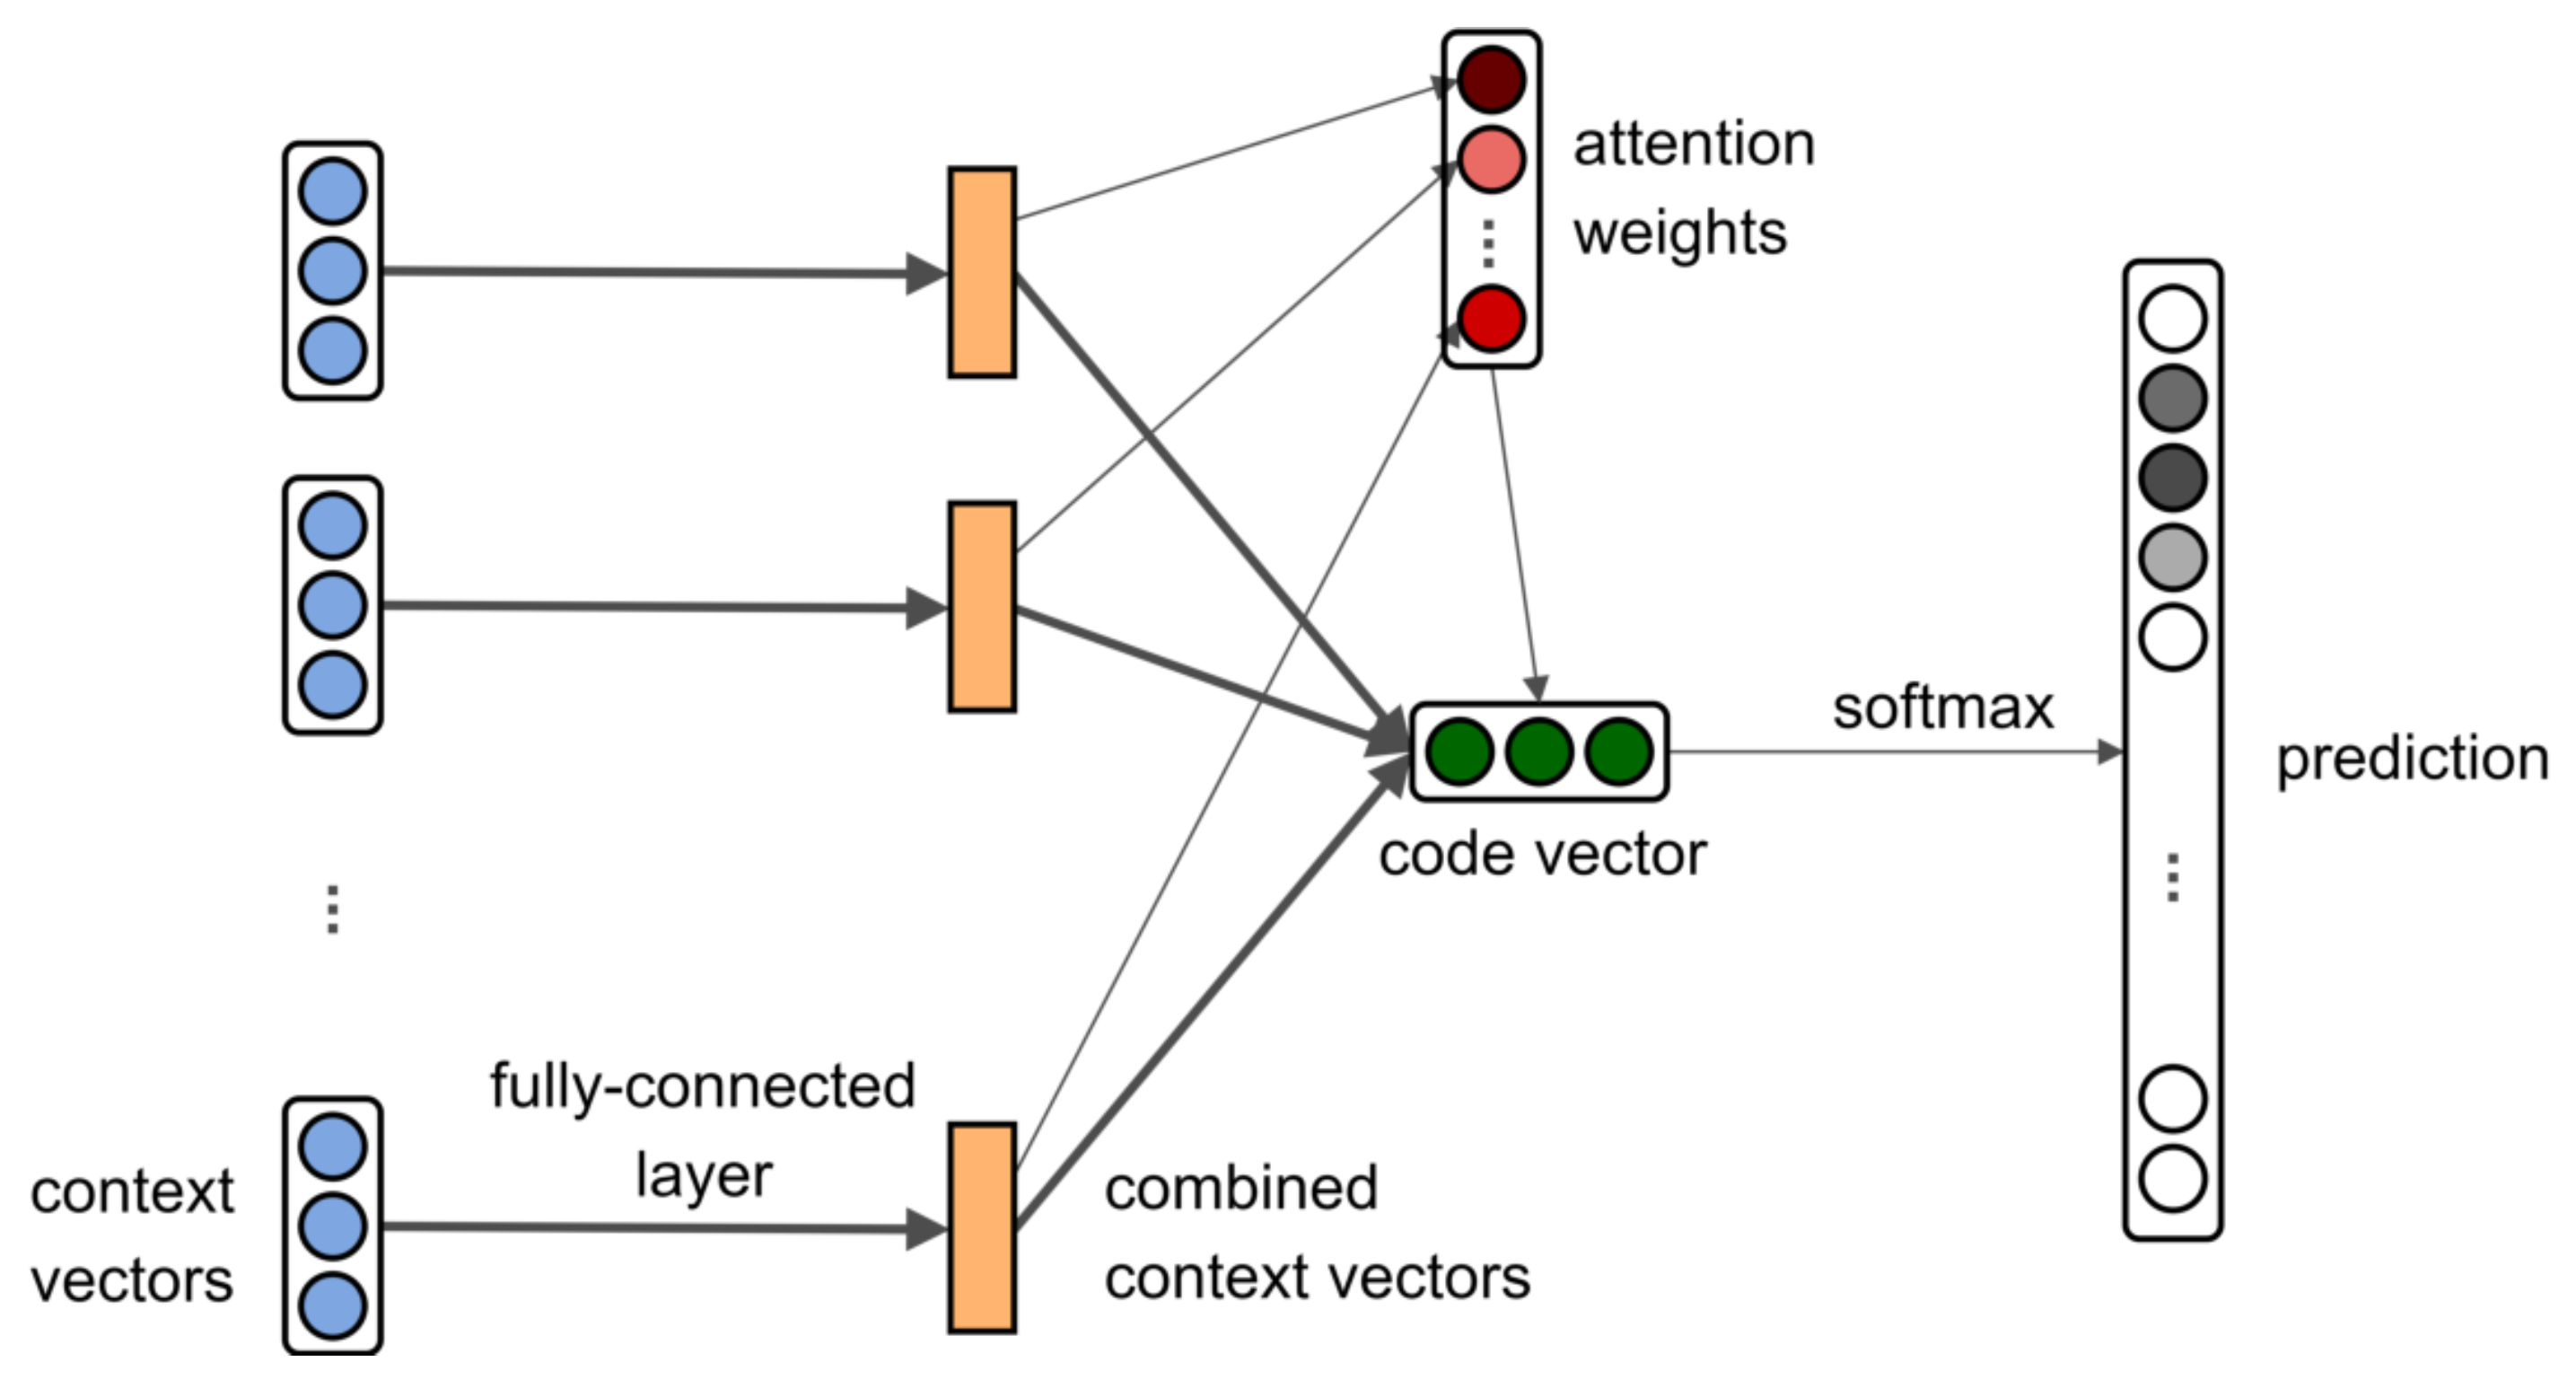
\includegraphics{images/code2vec_arch.png}
 }
 \caption[]{Code2vec architecture. Alon et al. \cite{alon2019code2vec}}
    \label{fig:code2vec_arch}
\end{figure}
 

\subsection{Training and prediction}
% detailed explanations in step:
% - representation idea (ast, path learning)

% - semantic labeling

% - SATD/fixed

% The model used is called code2vec. The idea is to represents source code snippets using a fixed-length vector i.e. code embedding. 
% The abstract syntax tree (AST) is used, there is an attention mechanism and it was successful in predicting semantic labeling.

% Simple and fast
The code-vector is used as input for a binary classifier. During the training, the model learns how to classify two classes: SATD and fixed. 
In the prediction phase it will calculate the probability that a specific class should be assigned to the given method body. 

%3.3
\section{Hyperparameter Tuning}

This section describes the process of tuning the hyperparameters of the model.

The initial experiments led us to quickly understand that using shorter snippets yielded better performances.
For example, a dataset with snippets shorter than 25 tokens has 4,256 samples and gives a 73\% test accuracy.
A dataset with snippets shorter than 200 tokens has 106,272 samples and gives a 58\% test accuracy. 


Using a smaller set of the dataset decreases the usefulness of the trained model because of less capability in generalization.
For the tuning of the hyperparameters, we empirically defined them to keep those snippets with less than 200 tokens; an example of a method composed of 199 tokens is shown in listing \ref{lst:snippet199}.

\begin{lstlisting}[caption={Code snippet with 199 tokens}, label={lst:snippet199},language=Java]
private CompoundWorkflow finishCompoundWorkflow(
  WorkflowEventQueue queue,
  CompoundWorkflow compoundWorkflow, 
  String taskOutcomeLabelId, 
  String userTaskComment, 
  boolean finishOnRegisterDocument, 
  List<NodeRef> excludedNodeRefs) {
    if ((finishOnRegisterDocument &&
      compoundWorkflow.isStatus(Status.FINISHED)) ||
      (!finishOnRegisterDocument &&
      checkCompoundWorkflow(compoundWorkflow,
      Status.IN_PROGRESS, 
      Status.FINISHED) == Status.FINISHED)) {
        if (log.isDebugEnabled()) {
            log.debug("--##string##--" + compoundWorkflow);
        }
    } else {
        setWorkflowsAndTasksFinished(queue, compoundWorkflow, 
            taskOutcomeLabelId, userTaskComment,
            finishOnRegisterDocument, excludedNodeRefs);
        if (finishOnRegisterDocument || excludedNodeRefs != null) {
            stepAndCheck(queue, compoundWorkflow);
        } else {
            stepAndCheck(queue, compoundWorkflow, Status.FINISHED);
        }
        boolean changed = saveCompoundWorkflow(queue,
            compoundWorkflow, null);
        if (log.isDebugEnabled()) {
            log.debug("--##string##--" + compoundWorkflow);
        }
    }
    CompoundWorkflow freshCompoundWorkflow =
        getCompoundWorkflow(compoundWorkflow.getNodeRef());
        
    if (!finishOnRegisterDocument && excludedNodeRefs == null) {
        checkCompoundWorkflow(freshCompoundWorkflow, Status.FINISHED);
    }
    checkActiveResponsibleAssignmentTasks(
        freshCompoundWorkflow.getParent());
    return freshCompoundWorkflow;
}
\end{lstlisting}

\noindent We based the tuning operation on these three hyperparameters:
\begin{itemize}
    \item default\_embeddings\_size: this value defines the length of the code vector, i.e. the vector representation of the snippet (see section \ref{sec:attention_code_vector}).
    \item max\_contexts: it is the maximum number of AST-paths used by the model (see section \ref{sec:code2vec_ast_paths}).
    \item dropout\_keep\_rate: the dropout is a random removal of neurons to prevent excessive adaptation to the training values and in so doing, reduce the likelihood of the network overfitting.
\end{itemize}

To explore the best values for these parameters we created a distributed experiment using Google Colab Pro and a tool called Optuna . 

\textbf{Optuna} is defined as ``A next-generation hyperparameter optimization framework''. It is capable to construct the parameter search space dynamically and it implements both searching and pruning strategies \cite{optuna_2019}. The initial experiments were conducted with a competing tool, Hyperopt \cite{bergstra2013making}, but it was abandoned in favor of Optuna.

\begin{figure}
 \centering
 \resizebox{\columnwidth}{!}{
  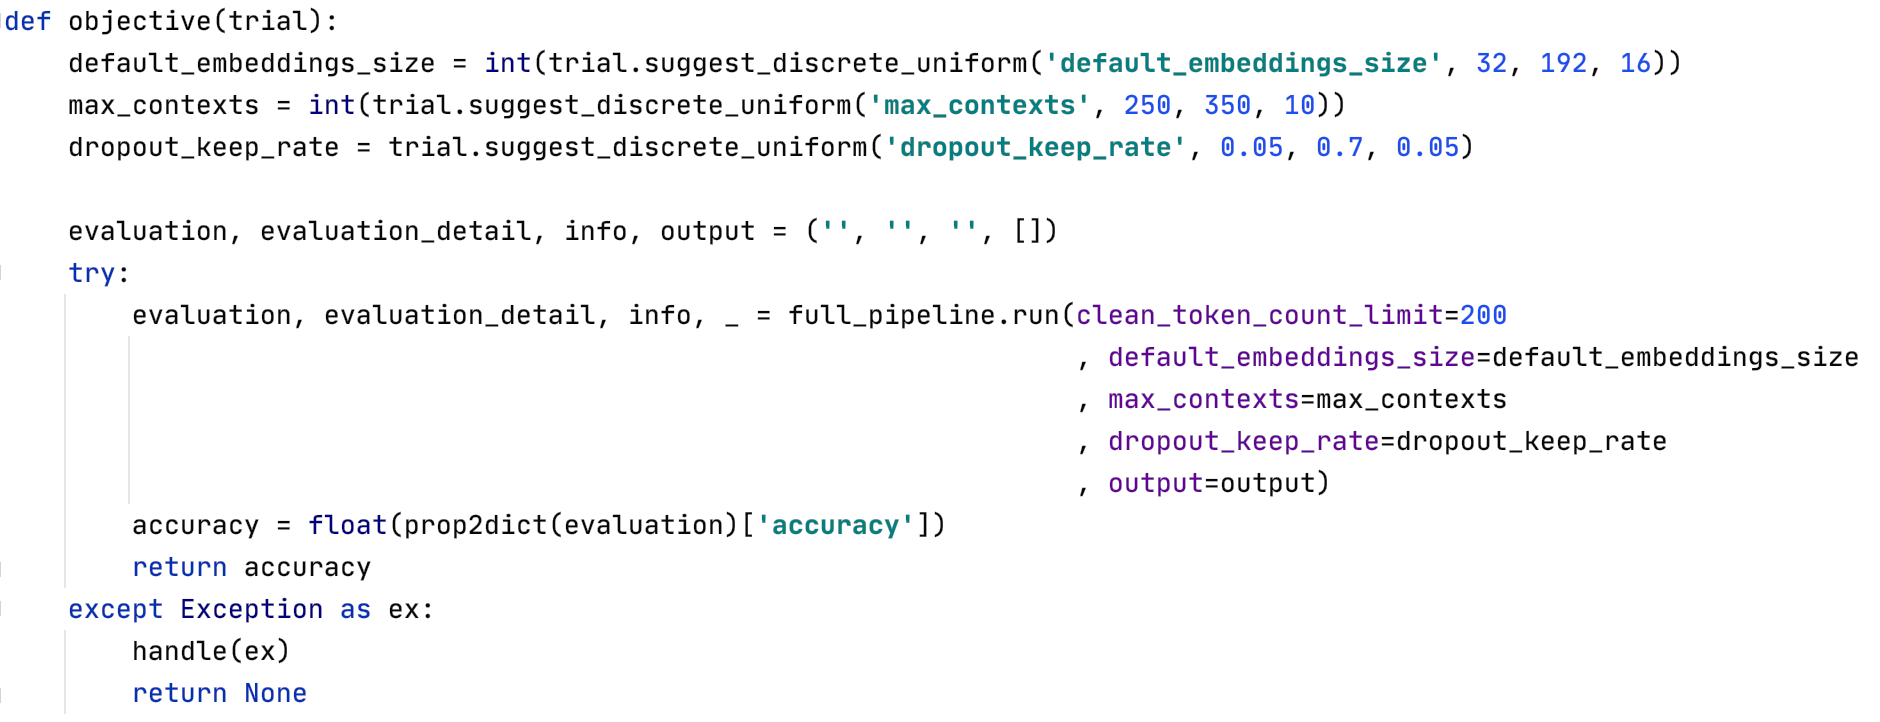
\includegraphics{images/optuna_objective.png}
 }
 \caption[]{Simplified version of the objective function - optuna\_worker.py}
    \label{fig:optuna_objective}
\end{figure}

The Optuna distributed worker was easier to setup and the distributed experiment gave less friction than Hyperopt. Figure \ref{fig:optuna_objective} shows a simplified version of the objective function required by Optuna where we define the search space for each hyperparameter. Our objective value is the test prediction accuracy.

The first rounds of experiments yielded good values for max\_contexts parameter: we found that the optimal value lies between 250-300. The other two parameters, default\_embeddings\_size and dropout\_keep\_rate, needed a different search space: figure \ref{fig:optuna_first} clearly shows the first two value bubbles crushed on the left. This suggested a new experiment with a different value search window shown in figure \ref{fig:optuna_second}. 

\begin{figure}
 \centering
 \resizebox{\columnwidth}{!}{
  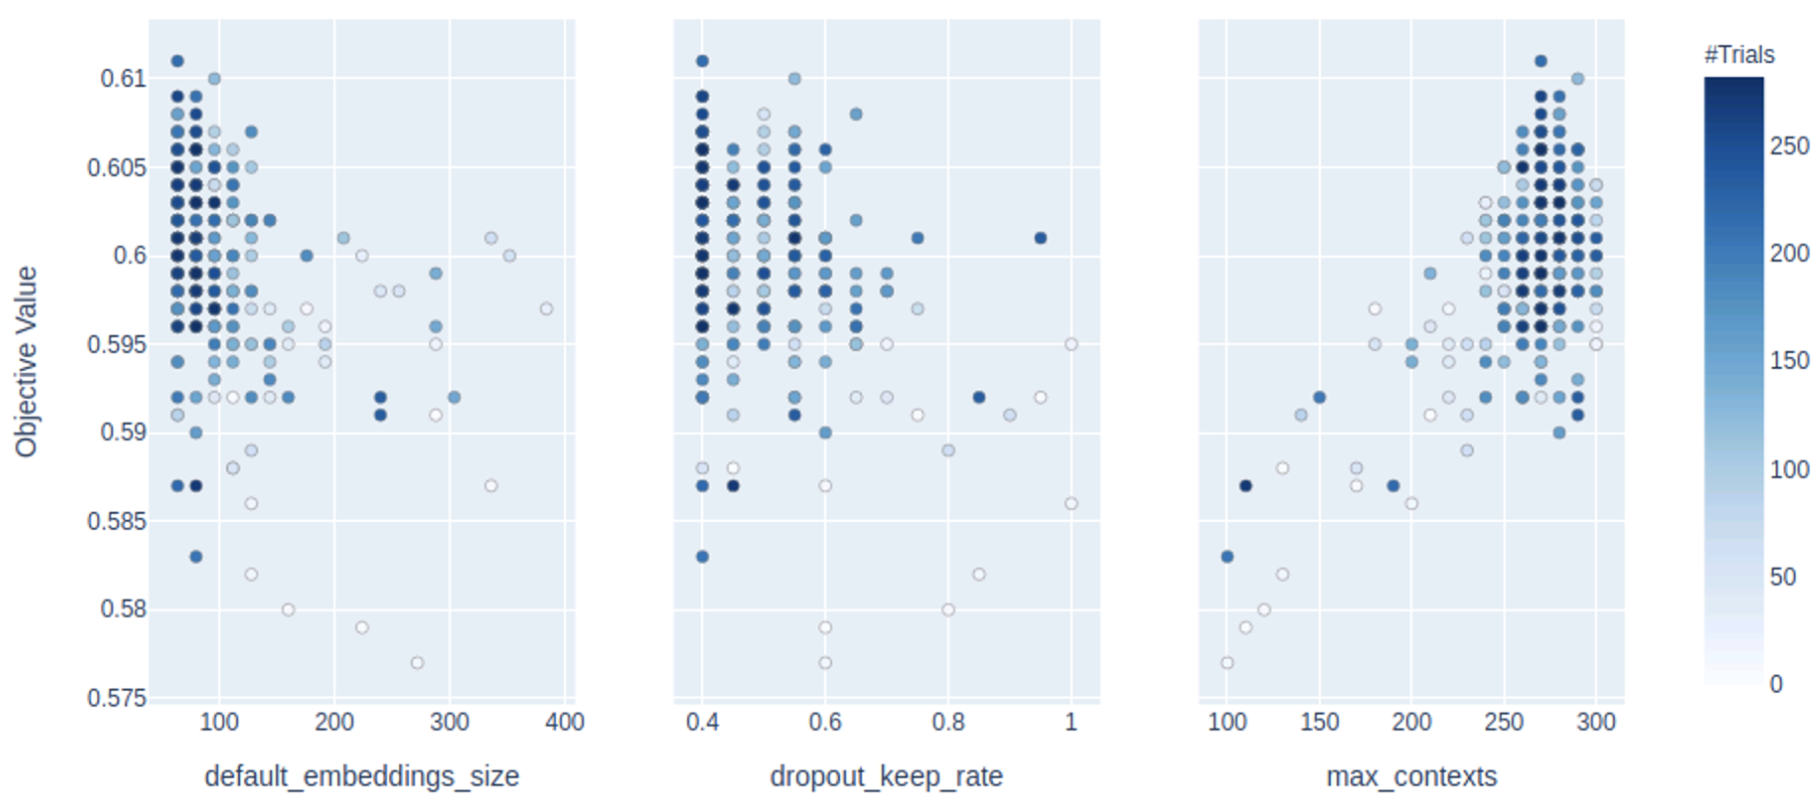
\includegraphics{images/optuna_first.png}
 }
 \caption[]{Slice plot for first grid search experiment}
    \label{fig:optuna_first}
\end{figure}


\begin{figure}
 \centering
 \resizebox{\columnwidth}{!}{
  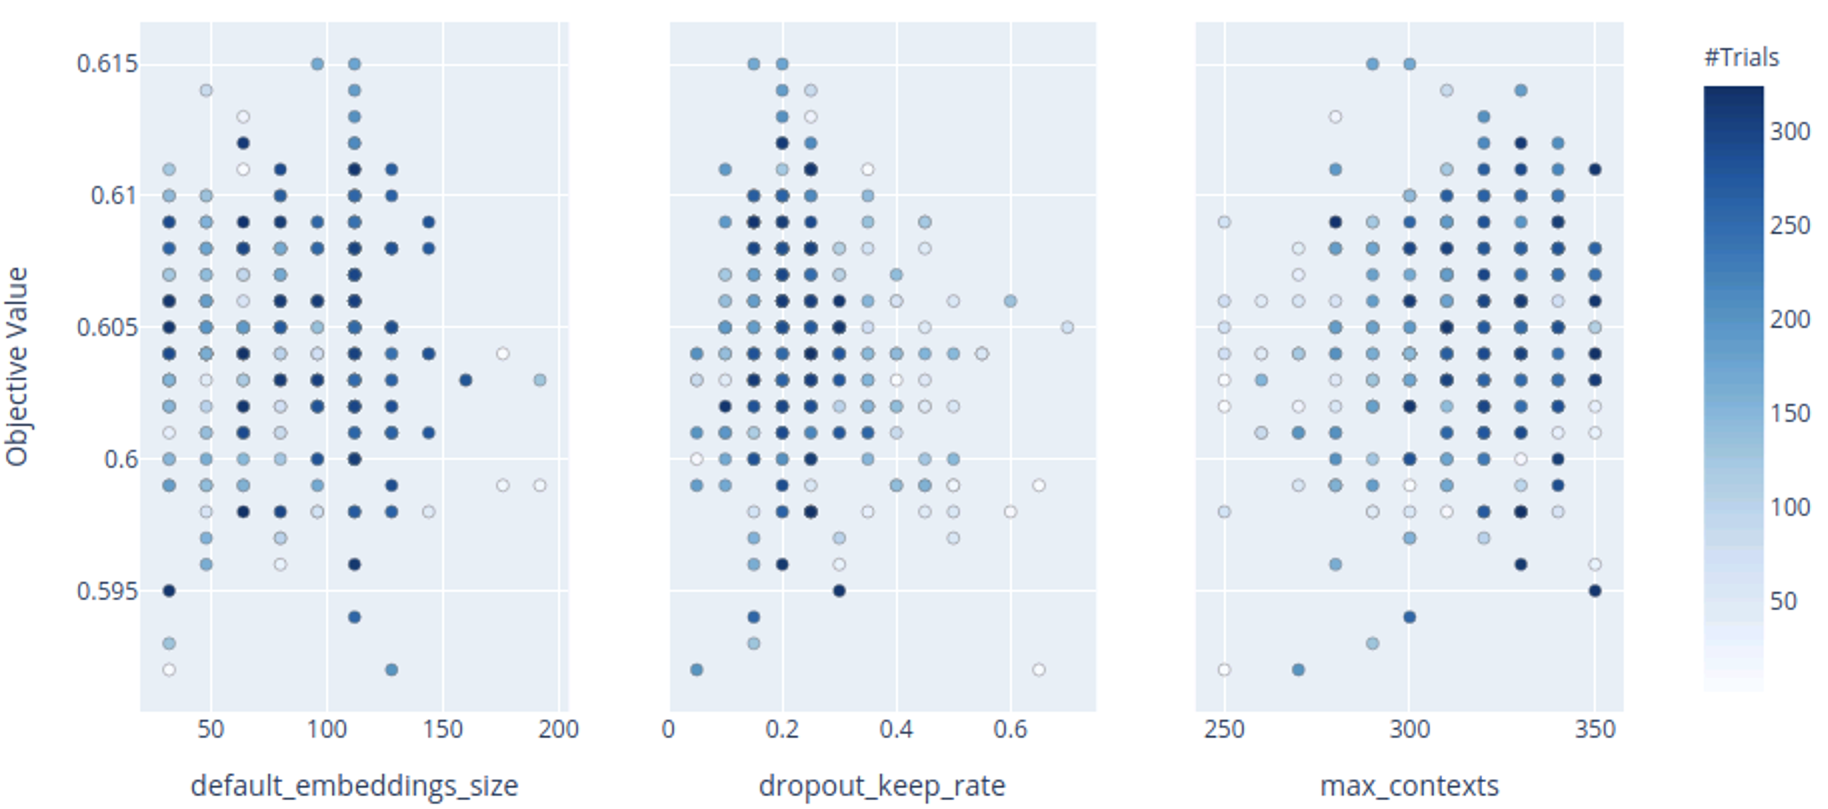
\includegraphics{images/optuna_second.png}
 }
 \caption[]{Slice plot for second grid search experiment with a centered search space}
    \label{fig:optuna_second}
\end{figure}



\textbf{Google Colab Pro.} The distributed experiment was executed on Google Colab infrastructure. We used 12 concurrent sessions, both with GPU and CPU. The Python notebook contained only a few lines of code (see listing \ref{lst:colab}). The first operation was to clone the GitHub repository with the source code for the distributed experiment. The second task was to invoke a Python function to setup the Colab environment: download PostgreSQL binaries, download and restore the backup with the dataset, install all the code2vec libraries and dependencies. The third and last step starts the Optuna worker. The results were stored in a central database as per Optuna design.

\begin{lstlisting}[caption={Google Colab notebook code}, label={lst:colab},language=Python]
    !cd /content; cd code2vec-satd-classifier && git pull || git clone \\
               https://github.com/simonegiacomelli/code2vec-satd-classifier
    %cd /content/code2vec-satd-classifier/code2vec-satd
    import satd_colab_starter as starter; starter.main()
    !python3 optuna_worker.py

\end{lstlisting}


% best satd-6 trial_id=37906,37915 0.615% accuracy
\noindent The best hyperparameters configuration found was the following:
\begin{itemize}
    \item default\_embeddings\_size: 112
    \item max\_contexts: 290
    \item dropout\_keep\_rate: 0.2
\end{itemize}
This setup raised the accuracy to 61.5\%.

\begin{figure}
 \centering
 \resizebox{\columnwidth}{!}{
  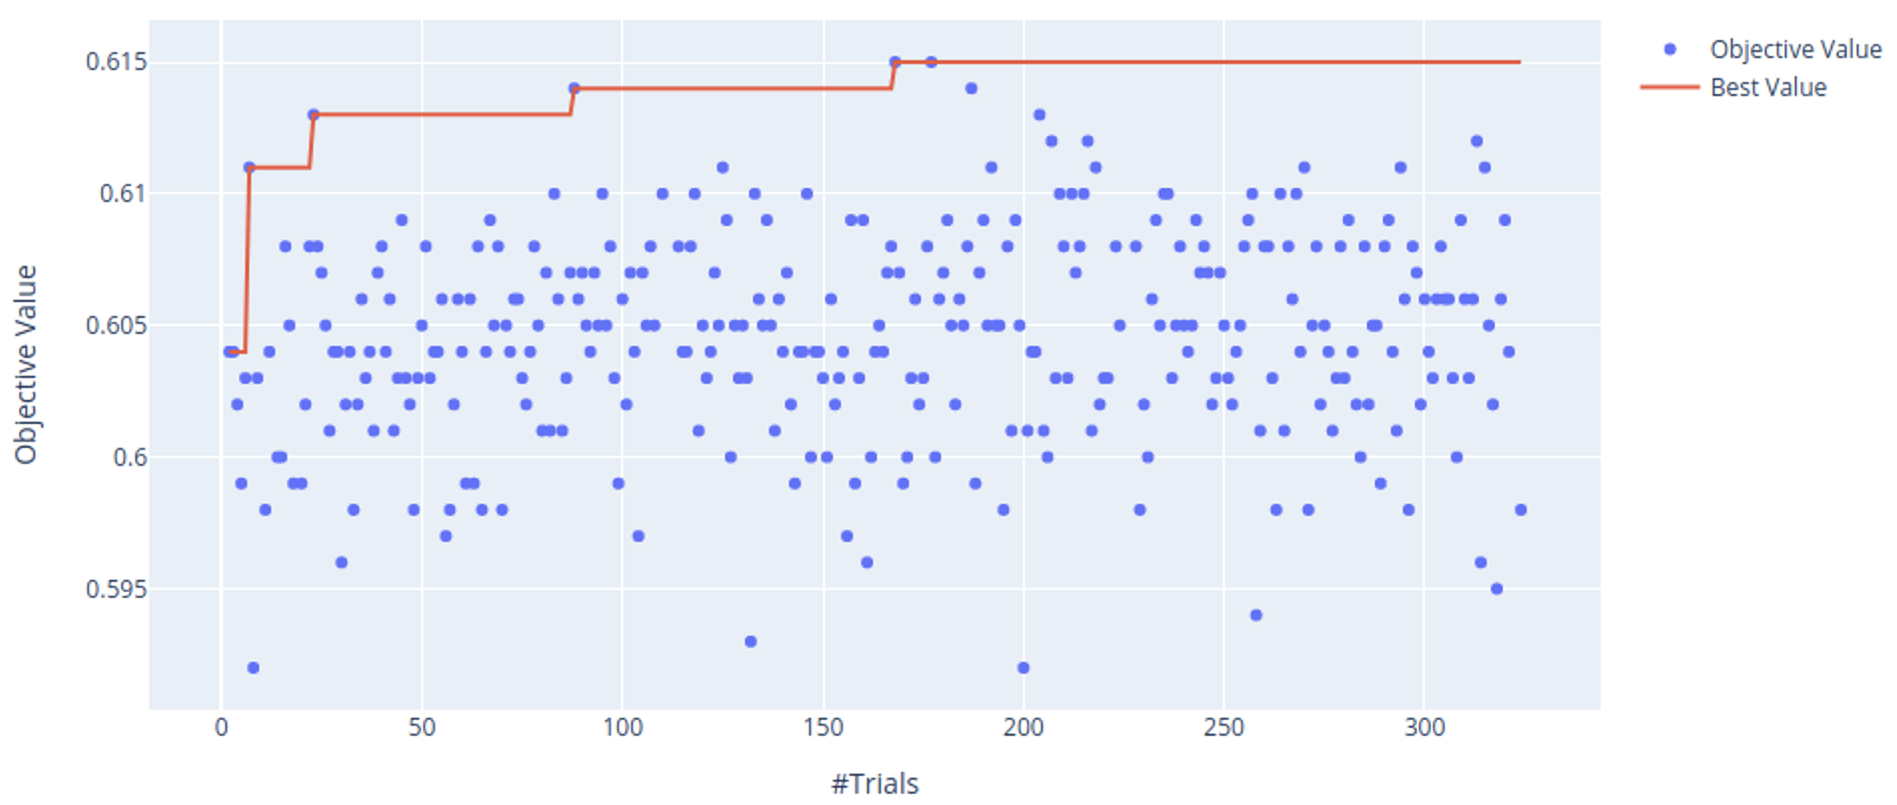
\includegraphics{images/optuna_history.png}
 }
 \caption[]{Second grid search experiment optimization history plot}
    \label{fig:optuna_second}
\end{figure}

